\section{实验效果}

本实验通过设计不同信道条件下的通信系统,评估了海明码编解码、交织解交织、QPSK调制方式以及高斯噪声信道对系统性能的影响。实验环境涵盖了无噪声理想信道、突发连续错误信道和高斯噪声干扰信道。

\subsection{无噪声理想信道}

首先我们设计了无噪声、无突发错误的理想信道条件,以验证系统基本功能的正确性。

通过实验设置中的开关(图 \ref{fig:result_noise_0}),我们可以手动输入任意16比特的信号,其中每个开关的上拨表示1,下拨表示0。每次按下重置键后,输入信号通过系统进行处理,并通过16个LED灯输出,灯亮表示1,熄灭表示0;注意本实验没有用到数码管。

从实验结果可见,输入信号与输出信号完全一致,验证了系统在理想条件下能够完美实现信号传输。

\begin{figure}[ht]
    \centering
    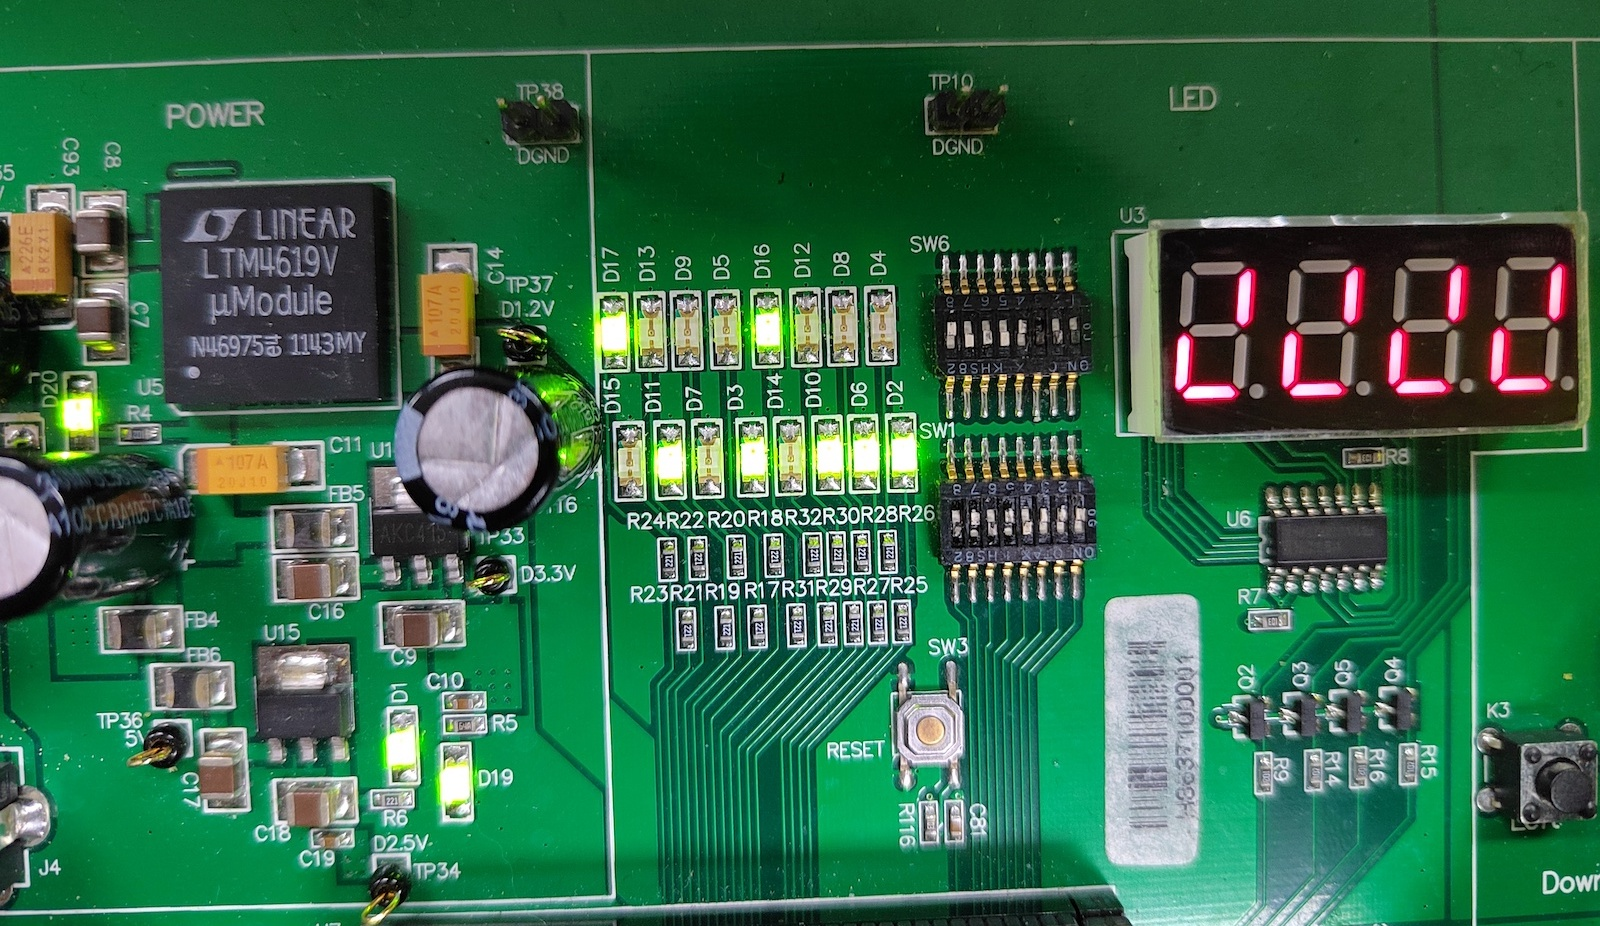
\includegraphics[width=.8\textwidth]{static/result_noise_0.jpg} 
    \caption{无噪声系统传输结果}\label{fig:result_noise_0}
\end{figure}

\subsection{突发连续错误}

接着,为了验证海明码、交织的功能,我们为输入信号加入了突发连续错误。

突发错误通常会导致多个连续比特发生错误,严重影响接收信号的准确性。为了模拟这一情况,我们通过编写代码引入连续错误,从而模拟信号中出现突发错误的情形。具体来说,突发错误通过以下代码实现:

\begin{codeblock}{verilog}
wire [27:0] inter_res_error;
assign inter_res_error =  {!inter_res[27], !inter_res[26], !inter_res[25], !inter_res[24], inter_res[23:0]};

...

case (qp_cnt)
    1: qpsk_in <= inter_res_error[1:0];
    2: qpsk_in <= inter_res_error[3:2];
    3: qpsk_in <= inter_res_error[5:4];
    4: qpsk_in <= inter_res_error[7:6];
    5: qpsk_in <= inter_res_error[9:8];
    6: qpsk_in <= inter_res_error[11:10];
    7: qpsk_in <= inter_res_error[13:12];
    8: qpsk_in <= inter_res_error[15:14];
    9: qpsk_in <= inter_res_error[17:16];
    10: qpsk_in <= inter_res_error[19:18];
    11: qpsk_in <= inter_res_error[21:20];
    12: qpsk_in <= inter_res_error[23:22];
    13: qpsk_in <= inter_res_error[25:24];
endcase
\end{codeblock}

代码中从第24位开始,连续4位的比特被反转,模拟了一个突发错误。

为了应对突发错误,通常可以采用海明码进行错误检测与纠正,并结合交织技术来增强系统的抗干扰能力。交织技术通过重新排列数据比特,将连续错误分布得更加均匀,从而减轻了多个连续错误对系统性能的影响。经过交织处理后,信号传输至接收端,接收端利用海明码对错误进行检测与纠正。海明码能够有效纠正单个比特错误,结合交织技术后,系统在处理多个连续错误时展现出了显著的恢复能力。

实验表明,经过海明码和交织技术的处理,接收端成功恢复了原始信号,证明了这两种技术在面对突发连续错误时具有良好的性能,显示了系统的可靠性。实验结果与图 \ref{fig:result_noise_0} 相同,此处不再重复展示。

图 \ref{fig:wave} 展示了信号在通过解交织器前后的波形图,可以看到 bit 串经过了解交织器的重新排列,使得连续突发错误被分散到多个待解码串中。

\begin{figure}[ht]
    \centering
    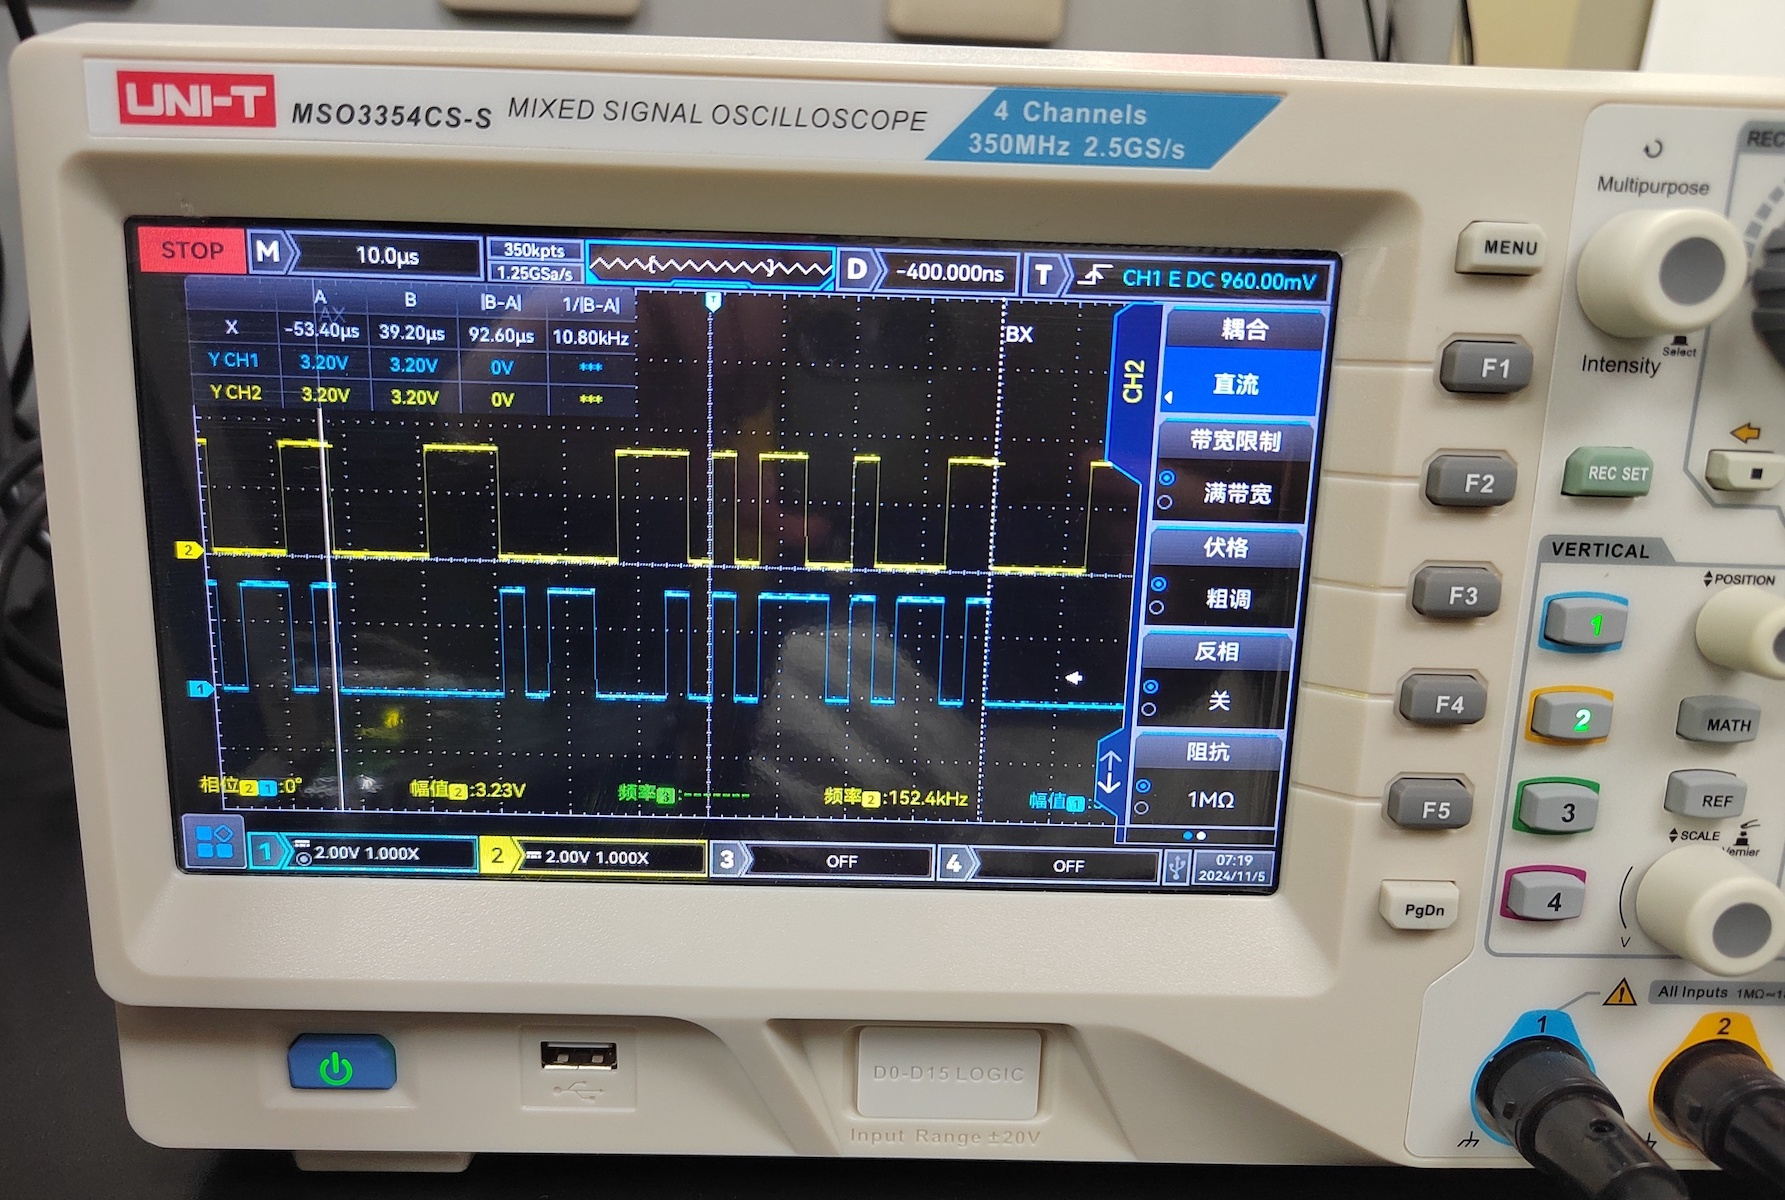
\includegraphics[width=.8\textwidth]{static/wave.jpg} 
    \caption{通过解交织器前后的信号波形}\label{fig:wave}
\end{figure}

\subsection{高斯噪声信道}

为全面评估系统在不同信道条件下的性能,我们还模拟了高斯噪声信道。通过调整高斯噪声的功率,模拟噪声功率对误码率(BER)的影响。实验结果表明,在理想信道条件下,系统的误码率接近零;而在高斯噪声影响下,随着噪声功率的增大,误码率逐渐增高。

表 \ref{tab:ber_results} 展示了不同信道条件下的误码率变化,表明噪声功率对系统性能具有重要影响,尤其在较低信噪比(SNR)下,系统的误码率显著增加。

\begin{table}[h!]
    \begin{center}
        \begin{tabular}{c|c|c}
        \hline
        \textbf{噪声相对功率} & \textbf{误码比例} & \textbf{误码率百分比}\\
        \hline
        1/4 & 0/16 & 0\%\\
        7/16 &  3/16 & 19\%\\
        1/2 & 4/16 & 25\%\\
        1 & 4/16 & 25\% \\ \hline
        \end{tabular}
        \caption{不同噪声(相对)功率下的误码率}\label{tab:ber_results}
    \end{center}
\end{table}
\begin{figure}[h!]
    \begin{center}
        \begin{minipage}{0.48\linewidth}
    		\centerline{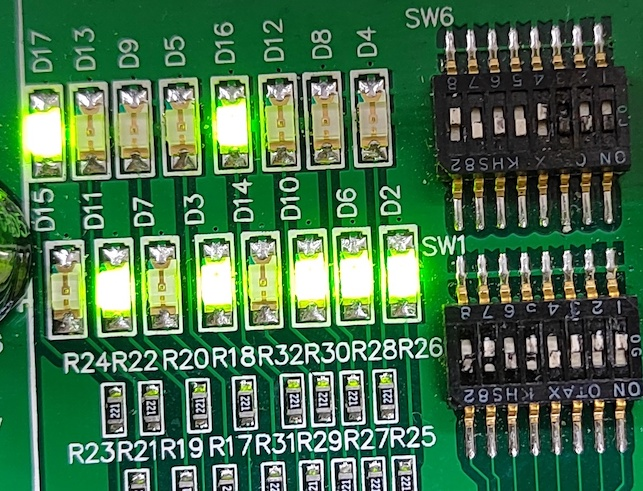
\includegraphics[width=\textwidth]{static/result_noise_1_256.jpg}}
    		\centerline{1/4 噪声,无错误}
    	\end{minipage}
        \hfill
    	\begin{minipage}{0.48\linewidth}
    		\centerline{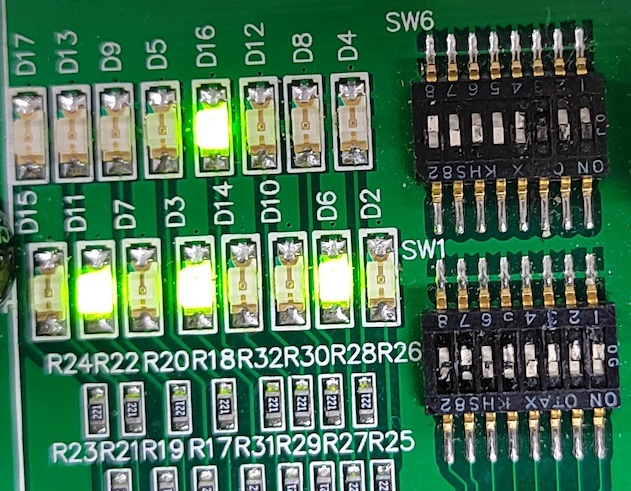
\includegraphics[width=\textwidth]{static/result_noise_7_16.jpg}}
    		\centerline{7/16 噪声,3 位误码}
    	\end{minipage}
        \\
    	\begin{minipage}{0.48\linewidth}
    		\centerline{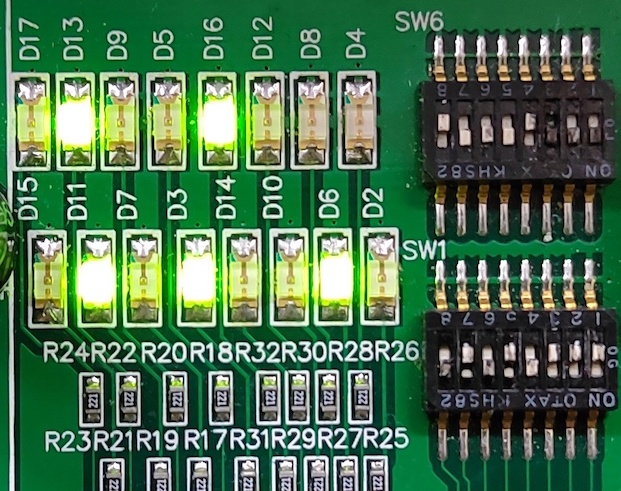
\includegraphics[width=\textwidth]{static/result_noise_1_2.jpg}}
    		\centerline{1/2 噪声,4 位误码}
    	\end{minipage}
        \hfill
        \begin{minipage}{0.48\linewidth}
    		\centerline{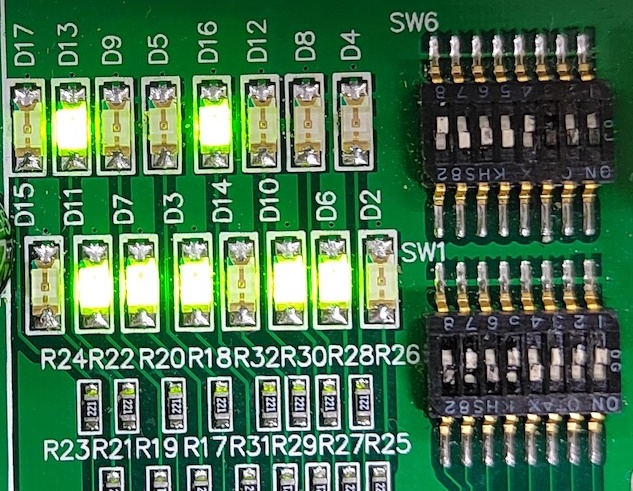
\includegraphics[width=\textwidth]{static/result_noise_1_1.jpg}}
    		\centerline{1 噪声,4 位误码}
    	\end{minipage}
    	\caption{不同噪声(相对)功率下的误码情况}
    	\label{fig:ber_results}
    \end{center}
\end{figure}

\subsection{总结}

通过本实验,我们综合评估了海明码、交织技术、QPSK调制和高斯噪声信道对通信系统性能的影响。在无噪声理想信道下,系统能够实现几乎完美的信号传输;在突发错误信道中,海明码和交织技术的结合有效降低了误码率,恢复了原始信号;而在高斯噪声信道下,增加信噪比是提高系统性能、降低误码率的关键因素。

实验结果表明,交织技术在面对突发错误时有显著的性能提升作用,而海明码和交织技术的结合能有效提高系统的可靠性。此外,高斯噪声对系统性能的影响较大,因此提高信噪比仍是应对噪声干扰的主要手段。

本次实验也加深了我们对通信实验技能的掌握,在动手实践的过程中我们逐步熟悉了verilog的语法细节、测试文件的编写、仿真和烧录的方法等等。在此感谢老师、助教和同学在我们实验过程中耐心的答疑解惑,让我们能够圆满完成此次实验。